
We are interested in two questions:
\begin{itemize}
\item Is it possible to learn an embedding of video frames in a self-supervised manner using only videos from a single viewpoint?
\item Is the learned embedding robust and well-behaved enough to power a reward function to use as part of a reinforcement learning problem?
\end{itemize}

\subsection{Embedding frames of a robotic arm}

We created 200 videos of a robotic arm performing trajectories in a simulated environment. The arm is initialized to random joint positions and it moves to goal joint positions which are also randomly sampled. We use the Bullet 3 physics simulator and a robot modelled after the Kuka iiwa robotic arm.

{
    \label{example-snap}
    \centering
    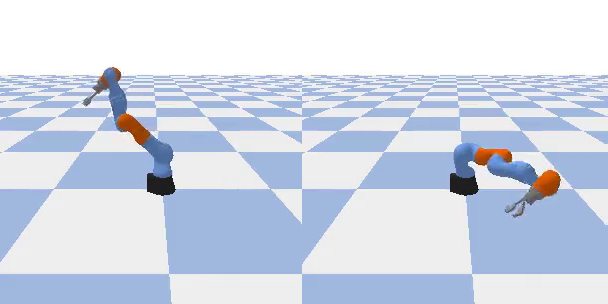
\includegraphics[width=8cm]{example_snap.png}
    \captionof{figure}{Two example frames from a recorded trajectory. The left frame is the goal position and the right frame is the start position.}
    \vspace{0.5cm}
}

We split the 200 videos such that 190 are used for training and 10 for validation.

We use a convolutional neural network derived from the Inception architecture as presented in \citep{inception-v3}. We use the 8 first layers of the network up until the layer labeled `Mixed\_5d`. We add two batch normalized convolutional layers, one spatial softmax transformation followed by two fully connected layers. This is very similar as the network used in \cite{self-supervised-learning}.

We implemented the neural network using the PyTorch deep learning framework \citep{pytorch}. The layers taken from the inception architecture are initialized to values pretrained on the ImageNet dataset. The added layers are randomly initialized using the default initialization scheme of the PyTorch package.

In our experiments, the output of the network is a 32-dimentional embedding constrained to have an $L_2$ norm of 10. The scaling factor of 10 was motivated by results presented in \cite{constrained-softmax-loss}. We use a margin value of 2.0. The positive frame was sampled from within 10 frames of the anchor frame. The negative frame was sampled from outside a range starting from 30 frames before the anchor frame and ending 30 frames after the anchor frame. The size of a video frame is 299 pixels in width and height.

We use the triplet loss presented in the previous section. At each epoch, we create a dataset of triplets sampled from 5 videos with 200 samples per video. We then run stochastic gradient descent with momentum against the triplet loss over this dataset 5 times after which a new triplet dataset is sampled and the process is repeated. The use a minibatch size of 64 triplets.

We use a learning rate schedule such that we start with a learning rate of 0.1. Each 500 epochs we decrease the learning rate to 1/10th of the previous rate until we reach 0.0001 inclusive. Table \ref{cnn-params} summarises the final parameters we used after tuning. The training of the network was performed on a single NVidia Quadro P5000 GPU.

{
    \vspace{0.5cm}
    \centering
    \begin{tabular}{@{}ll@{}}
    \toprule
    \textbf{Parameter}             & \textbf{Value}    \\ \midrule
    \textbf{minibatch size}        & 64                \\
    \textbf{learning rate}         & 0.1-0.0001        \\
    $\boldsymbol{\delta}$                & 2.0               \\
    \textbf{positive frame margin} & 10                \\
    \textbf{negative frame margin} & 30                \\
    \textbf{optimizer}             & SGD with momentum \\
    \textbf{momentum}              & 0.9               \\
    \textbf{embedding dimensions}  & 32
    \end{tabular}
    \captionof{table}{The parameters we used for training our embedding function.}
    \label{cnn-params}
}

\subsection{Learning to imitate}

We used the learned embedding to teach the same simulated robot to imitate itself in a video performing different trajectories. We use the proximal policy optimization algorithm to optimize the loss function.

The observation at each time step is a concatenation of the robot joint states, joint velocities, the TCN embedding of an image of itself and the TCN embedding of the next video frame at that timestep.

The reward is calculated using the huber loss presented in section \ref{sec:methods} using the embedding of an image of the robot and the embedding of an example video frame. Actions are torques applied to the 7 joints of the robotic arm. The 5 joints of the end effector were left out to simplify the learning problem.  

The output of the policy network is a 7-dimensional vector. The continuous vector values determine forces of the motors and the values are between -200 and 200. \textit{Hyperbolic tangent function} is used an the activation function for the hidden units in the fully connected policy network. We experimented different layer structures for the learning problem. As the complexity of the action space is high, the best result was achieved with 3 hidden layers with width 128. The same input value is used for the value network. The network returns recommendation of the state in scalar. The value network share the same features as the policy network but it has 2 hidden layers.

We trained the imitation agent by running 16 processes of the simulation in parallel. We evaluate the policy network to get an action for each process at each time step. We use a rollout storage to sample updates from. An update is done on the policy and value networks every 1000 time steps by sampling minibatches from the rollout storage. All the parameters we used are summarized in table \ref{ppo-params}.

{
    \vspace{0.5cm}
    \centering
    \begin{tabular}{@{}ll@{}}
    \toprule
    \textbf{Parameter}             & \textbf{Value}    \\ \midrule
    $\boldsymbol{\gamma}$        & 0.99                \\
    $\boldsymbol{\tau}$        & 0.95                \\
    clip $\boldsymbol{\epsilon}$        & 0.2                \\
    learning rate                       & 0.0007 \\
    optimizer                        & Adam \\
    epochs each update        & 4                \\
    update interval        & 1000 time steps                \\
    \end{tabular}
    \captionof{table}{The parameters we used for proximal policy optimization.}
    \label{ppo-params}
}
